\chapter{Nachtisch}
\section{Rosa Wölkchen}\index{Rosa Wölkchen}\index{Weihnachtsklassiker!Rosa Wölkchen}
\subsection*{Zubereitung}
\begin{tabular}{lrr}
	Personen         &                        6 &  \\
	Zubereitungszeit &                       30 & Minuten \\
	Gesamtzeit       &                        8 & Stunden \\
	Entnommen aus    & \cite{AnnetteWolter1998} &
\end{tabular} 

\subsection*{Zutaten}
\begin{tabular}{lrr}
	Gelantine            &   7 & Blatt \\
	Erdbeeren            & 250 &     g \\
	Zucker               &  75 &     g \\
	Vanillezucker       &   2 &    EL \\
	Sahne                & 0,5 &     l \\
	Vollmilchjoguhrt     & 150 &     g \\
	ungespritzte Zitrone &   1 &  \\
	Puderzucker          &     &
\end{tabular} 

Die Gelatine in kaltem Wasser einweichen. Erdbeeren (falls nicht gefroren, waschen und einige zur Garnitur kaltstellen, nicht in Zutaten enthalten) mit Zucker und Vanillezucker bestreuen und mit einer Gabel zerdrücken.

Die Hälfte der Sahne mit dem Joghurt schaumig rühren. Die Zitrone warm waschen und abtrocknen. Die Schale abreiben und den Saft auspressen. Den Zitronensaft erhitzen und die ausgedrückte Gelatine darin auflösen. 3 EL der Joghurtcreme unter den Zitronensaft mischen und diesen dann mit der Zitronenschale und der gesamten Creme verrühren. Die Creme kühl stellen, bis sie zu stocken beginnt.

Die restliche Sahne steif schlagen, mit dem Erdbeerpüree unter die Creme mischen. Die Masse im Kühlschrank fest werden lassen.  

\section{Zitronencreme}\index{Zirone!Creme}\index{Zitronen Creme} 
\subsection*{Zubereitung}
\begin{tabular}{lrr}
	Personen         &  4 &         \\
	Zubereitungszeit & 30 & Minuten \\
	Gesamtzeit       &  8 & Stunden \\
	Entnommen aus    &    &
\end{tabular} 

\subsection*{Zutaten}
\begin{tabular}{lrr}
	Gelantine            &   4 & Blatt \\
	Zucker               &  80 &     g \\
	Vanillezucker       &   1 &    Päckchen \\
	Sahne                & 0,25 &     l \\
	Vollmilchjoguhrt     & 250 &     g \\
	Abrieb ungespritzte Zitrone &   1 &  \\
	Zitronensaft & 75 &ml \\
	Crème frâiche          & 60	    & g
\end{tabular} 

Die Gelatine in kaltem Wasser einweichen. 

Joghurt, Crème frâiche, Vanillezucker und Zucker verrühren.

Gelatine ausdrücken und mit dem Zitronensaft erhitzen. Den Abrieb hinzugeben, unter die Creme rühren und kalt stellen.  

Wenn die Creme anfängt zu stocken, die geschlagene Sahne unterrühren. Zirka 8 Stunde kalt stehen lassen. Nach Lust mit Beeren und Schokladenstückchen garnieren.

\section{Crème Brulée}\index{Eier}\index{Sahne}
\subsection*{Zubereitung}
\begin{tabular}{lrr}
	Personen         &                        6 &  \\
	Zubereitungszeit &                       30 & Minuten \\
	Gesamtzeit       &                        8 & Stunden \\
	Entnommen aus    & \cite{Cre2015} &
\end{tabular} 

\subsection*{Zutaten}
\begin{tabular}{lrr}
	Sahne                  &          400 &       ml \\
	Milch                  &          200 &       ml \\
	Zucker                 &           90 &        g \\
	Vanilleschote          &            1 &  \\
	Vanillezucker, Bourbon &            1 & Päckchen \\
	Eigelb                 &          4-5 &  \\
	brauner Rohrzucker     & zu Bestreuen &
\end{tabular} 

Das Mark aus der Vanilleschote kratzen und mit etwas Zucker im Mörser innig vermischen. Sahne, Milch, Vanillezucker und den restlichen Zucker miteinander mischen und den Zucker auflösen. Die Eigelb dazu geben und kurz mit dem Stabmixer durchmixen. Die Mischung einige Stunden stehen lassen.

Die Eiersahne nochmals gut durchmischen, damit sich die Vanille gut verteilt, aber Achtung, die Flüssigkeit soll nicht schäumen. Die Eiersahne in die Förmchen gießen und diese in die Saftpfanne des Backofens setzen. In den auf 150 Grad (Umluft) vorgeheizten Backofen schieben, in die Saftpfanne kochend heißes Wasser gießen, so dass die Förmchen gut zur Hälfte im Wasser stehen. Wenn die Creme Blasen wirft, die Temperatur ggf. etwas herunterschalten. Nach 40 – 45 Minuten sollte die Creme fest sein (in der Mitte ist sie dann gerade nicht mehr flüssig).

Die Creme erkalten lassen und kurz vor dem Servieren dünn mit dem braunen Rohrzucker überstreuen und am Tisch mit einem Brenner karamellisieren lassen.

Das Geheimnis einer guten Crème Brulée liegt ausnahmsweise mal nicht beim genauen Einhalten des Rezeptes oder der Zubereitung. Der Qualität der Crème tut es keinen Abbruch, wenn mehr oder weniger Milch, ob 4 oder 6 Eigelb oder etwas mehr oder weniger Zucker verwendet werden. Eine gute Crème Brulée wird man nur in den entsprechenden Förmchen hinbekommen. Die Förmchen sollten nicht höher als 2,5 – 3 cm sein und nicht mehr als 12 cm im Durchmesser haben und am besten aus hitzebeständigen Porzellan bestehen. Bei größeren oder tieferen Gefäßen stockt die Crème nicht gleichmäßig, ist außen schon zu fest und innen noch zu flüssig, braucht Ewigkeiten zum Stocken oder braucht zu hohe Temperaturen und flockt dadurch aus.

\section{Panna Cotta}\index{Sahne}\index{Panna Cotta}
\todo[inline]{eigenes Bild und Soße}
\begin{figure}[H]
\centering
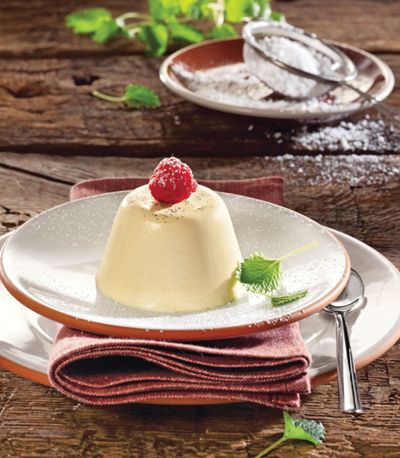
\includegraphics[width=0.4\linewidth]{Bilder/PannaCotta}
\caption{Panna Cotta}
\label{fig:PannaCotta}
\end{figure}

\subsection*{Zubereitung}
\begin{tabular}{lrr}
	Personen         &                        4 &  \\
	Zubereitungszeit &                       20 & Minuten \\
	Gesamtzeit       &                        8 & Stunden \\
	Entnommen aus    & \cite{Naumann2016} &
\end{tabular} 

\subsection*{Zutaten}
\begin{tabular}{lrr}
	Sahne         & 400 &   ml \\
	Zucker        &  40 &    g \\
	Vanilleschote &   1 &  \\
	Gelantine     &   3 & Blatt
\end{tabular} 


\begin{enumerate}
	\item Die Vanilleschote längs aufschneiden, das Mark mit einem spitzen Messer herauskratzen. Die Sahne mit dem Vanillemark, der Vanilleschote und dem Zucker in einer Schüssel im Wasserbad erhitzen und für mindestens 10 Minuten köcheln lassen.
	\item Die Gelatine in kaltem Wasser einweichen. Den Topf vom Herd nehmen, die Vanilleschote herausnehmen und die ausgedrückte Gelatine in die Sahne einrühren. Den Topf wieder auf den Herd stellen und die Gelatine auf kleiner Flamme unter Rühren auflösen.
	\item Dessertschalen mit kaltem Wasser ausspülen, die gekochte Sahne einfüllen und im Kühlschrank 4 – 5 Stunden erstarren lassen. Die Panna cotta vor dem Servieren auf Dessertteller stürzen und nach Belieben garnieren.
\end{enumerate}

\section{Mousse au Chocolat}\index{Sahne}\index{Mousse au Chocolat}\index{Eier!roh}


\subsection*{Zubereitung}
\begin{tabular}{lrr}
	Personen         &                        4 &  \\
	Zubereitungszeit &                       30 & Minuten \\
	Gesamtzeit       &                        6 & Stunden \\
\end{tabular} 

\subsection*{Zutaten}
\begin{tabular}{lrl}
	edle Zartbitterschokolade        &  2 & Tafeln \\
	Zucker                           & 50 & g      \\
	Sahne                            &  1 & Becher \\
	Wasser, Orangenlikör oder Cognac &  3 & EL \\	
	Espresso Pulver & 1& Portion
\end{tabular} 


\begin{enumerate}
	\item Für dieses Rezept muss zuerst die Schokolade in einem Wasserbad zum Schmelzen gebracht werden. Die Eier trennen nach Eiweiß. Das Eiweiß schaumig schlagen. Die Sahne sehr steif schlagen. Sahne und Eischnee kühl stellen.

	\item Aus dem Zucker, dem Eigelb und der Flüssigkeit wird eine schaumige Masse gerührt. In diese Masse wird die geschmolzene Schokolade und das Espresso Pulver gegeben und kräftig verrührt. Langsam das Eiweiß mit einem Schneebesen unter die braune Masse heben und danach die steif geschlagene Sahne.

	\item Die Mousse au Chocolat ist noch recht flüssig in ihrer Konsistenz, damit sie schön fest wird, sollten kleine Schalen für das Dessert bereit gestellt sein und die Masse wird portionsweise hinein gefüllt. Anschließend werden die gefüllten Dessertschalen für mindestens vier Stunden in den Kühlschrank gestellt, damit die Mousse au Chocolat ihre feste Konsistenz erhält. Vor dem Servieren werden die Dessertschalen rechtzeitig wieder aus dem Kühlschrank genommen, damit die Mousse au Chocolat fast die Zimmertemperatur annehmen kann. Jetzt ist das Dessert ein wahrer Gaumengenuss und zerschmilzt auf der Zunge. 
\end{enumerate}

\section{Omas Pudding in Tills Variante}\index{Speisestärke}\index{Sahne}\index{Pudding}\index{Vanille}


\subsection*{Zubereitung}
\begin{tabular}{lrr}
	Personen         &                        4 &  \\
	Zubereitungszeit &                       30 & Minuten \\
	Gesamtzeit       &                        4 & Stunden \\
\end{tabular} 

\subsection*{Zutaten}
\begin{tabular}{lrl}
	Milch        &  600 (700) & ml \\
	Sahne                            &  100 (0) & ml \\
	Zucker                           & 75 & g      \\
	Vanilleschote				& 1 &\\
	Vanillezucker & 1 & Päckchen\\
	Speisestärke                            &  45 & g \\
	Eier                            &  2 &   \\
	Erdbeeren, Himbeeren oder Johannisbeeren & & \\
\end{tabular} 


\begin{enumerate}
	\item 600 ml der Flüssigkeit mit der ausgekratzten Masse der Vanilleschote und der Vanilleschote aufkochen  und 30 Minuten ziehen lassen.
	\item Den Rest der Flüssigkeit mit der Speisestärke, dem Zucker und dem Eigelb glatt rühren.
	\item Eiweiß zu Schnee schlagen. 
	\item Die Flüssigkeit mit der gelben Masse noch mal aufkochen. Nach dem Stocken das Eiweiß unterrühren und dann über die geforrenen Früchte geben.
\end{enumerate}


\section{Jogurtbombe}\index{Joghurt}\index{Sahne}\index{Früchte}\index{Vanille}


\begin{figure}[H]
	\centering
	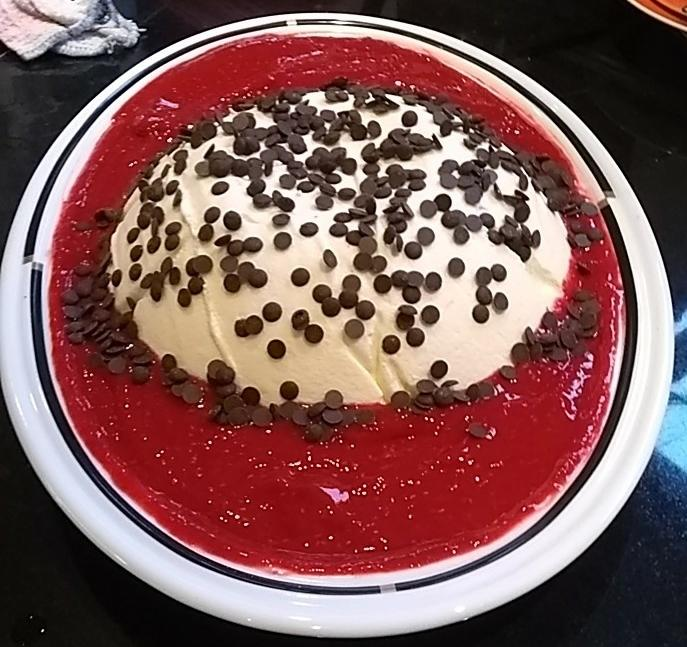
\includegraphics[width=0.46\linewidth]{Bilder/JogurtBombe}
	\caption{Jogurtbombe}
	\label{fig:Jogurtbombe}
\end{figure}



\subsection*{Zubereitung}
\begin{tabular}{lrr}
Personen         &                        6 &  \\
Zubereitungszeit &                       30 & Minuten \\
Gesamtzeit       &                        4 & Stunden \\
\end{tabular} 

\subsection*{Zutaten}
\begin{tabular}{lrl}
	Naturogurt                               & 750 & g        \\
	Sahne                                    & 600 & ml       \\
	Zucker                                   & 180 & g        \\
	Borbon-Vanillezucker                     & 1,5 & Päckchen \\
	Erdbeeren, Himbeeren oder Johannisbeeren & 400 & g
\end{tabular} 


\begin{enumerate}
\item Joghurt, Zucker und Vanille-Zucker verrühren. Steif geschlagene Sahne unterheben.
\item Ein Sieb imit Geschirrtuck auslegen und in eine größere Schüssel hängen, Die Masse einfüllen, mit Frischhaltefolie abdecken und z.b. mit einem Teller beschweren. Das ganze mindestens 12 Stunden kalt stellen, Zwischendurch die Flüssigkeit abgießen. 
\item Die Masse auf eine Platte stürzen und mit pürierten Früchten garnieren. Ggf. etwas Himbeergeist dazu geben.
\end{enumerate}

\section{Schoko-Soufflé}\index{Schokolade}\index{Schokolade!flüssig}\index{Soufflé}%https://www.chefkoch.de/rezepte/1326851237499511/Schoko-Souffle.html

%\begin{figure}[H]
%	\centering
%	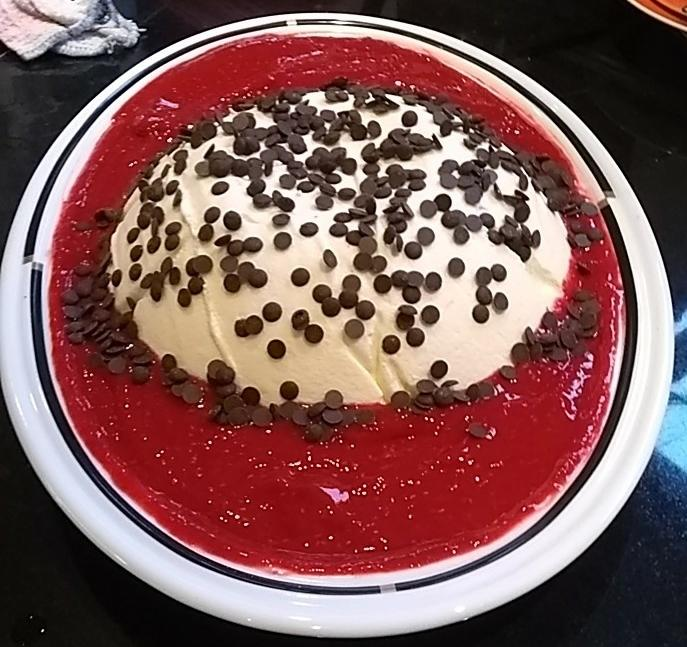
\includegraphics[width=0.46\linewidth]{Bilder/JogurtBombe}
%	\caption{Jogurtbombe}
%	\label{fig:Jogurtbombe}
%\end{figure}
%


\subsection*{Zubereitung}
\begin{tabular}{lrr}
	Personen         &       6 &         \\
	Zubereitungszeit &      30 & Minuten \\
	Ruhezeit         &      12 & Stunden \\
	Koch-/Backzeit   & ca.  13 & Minuten \\
	Gesamtzeit       &      14 & Stunden
\end{tabular} 

\subsection*{Zutaten}
\begin{tabular}{lrl}
	Eier                                                      &   2 &   \\
	Eigelb                                                    &   2 &   \\
	Zucker                                                    &  80 & g \\
	Mehl                                                      &  80 & g \\
	Kuvertüre, dunkle, besser 70 \% ige Edelbitter-Schokolade & 100 & g \\
	Butter, gewürfelt                                         & 100 & g \\
	Butter, für die Förmchen                                  &     &   \\
	Mehl, für die Förmchen                                    &     &   \\
	Kakaopulver, oder Puderzucker zum Bestreuen               &     &   \\
	Amaretto nach Belieben                                    &     &
\end{tabular} 


\begin{enumerate}
	\item Eier, Eigelb und Zucker in einer Schüssel schaumig schlagen, bis sich der Zucker gelöst hat. 
	\item Schokolade in einer Schüssel über dem Wasserbad schmelzen, dann die Butterwürfel zur Schokolade geben, unter Rühren auflösen und unterziehen (hier kommt dann evtl. auch der Amaretto rein). Die Masse zum Eier-Gemisch geben und unterziehen. Mehl sieben und vorsichtig unterheben.
	\item Förmchen mit Butter fetten und mit etwas Mehl ausstäuben. Die Förmchen zu zwei Dritteln mit der Soufflémasse füllen und über Nacht (12 Stunden) in den Tiefkühler stellen. Die Förmchen kurz vor dem Servieren in den auf 180 °C vorgeheizten Ofen schieben und bei Umluft 13 Minuten backen.
	\item Nach dem Backen die Soufflés vorsichtig aus der Form stürzen und auf Teller setzen. Mit Kakao oder Puderzucker bestäuben.
	\item Mit Vanillesauce oder Vanilleeis servieren. Die Soufflés sind allerdings mächtig genug.
	\item Tipp: Man kann die Soufflés auch länger im Tiefkühler lassen. Also ein Dessert, das sich gut vorbereiten lässt.
\end{enumerate}


\section[Orange Cheesecake Dessert]{Orange Cheesecake Dessert im Glas \textmd{(siehe \cite{sonjaOrangeCheesecake})}} \index{Cheesecake!Glas}
    Anstatt der Spekulatius habe ich Butterkekse (Vollkorn) verwendet. Mit unseren 100 ml Mini Weckgläser ergeben sich 9 Portionen.
    
    \subsection*{Zutaten}
    \textbf{Für die Sauce} \\
    \begin{tabular}{r l}
            180 g & frische Orange (geschält, ca. 1 große Orange)   \\
             50 g & Orangensaft oder Orangenlikör (z. B. Cointreau) \\
             24 g & Vanillesoßenpulver ohne Kochen                  \\
        ein wenig & geriebene Orangenschale
    \end{tabular}
    
    \textbf{Für die Creme}\\
    \begin{tabular}{r l}
           150 g & Mascarpone                                   \\
           250 g & Quark mit 20 \% Fett                         \\
            50 g & Honig                                        \\
        0.5–1 TL & Vanilleextrakt selbst gemacht oder gekauft   \\
           etwas & geriebene Orangenschale                      \\
           200 g & Schlagsahne                                  \\
            2 TL & Sahnesteif                                   \\
            1 EL & Puderzucker                                
    \end{tabular}
    
    \textbf{Außerdem} \\
    \begin{tabular}{r l}
         9 & Butterkekse Vollkorn einer pro Portion \\
         2 & Orangen-Scheibe (geviertelt für die Deko)\\
         9 & kleine Weckgläser á 200 ml
    \end{tabular}
    
    \subsection*{Zubereitung}
    \begin{itemize}
        \item Die Kekse zerbröseln und in 9 Weckgläser á 100 ml verteilen.
        \item Orange mit dem Orangensaft und Likör, Vanillesoßenpulver und ein wenig Orangenschale pürieren.
        \item Mascarpone und Quark mit dem Honig, Vanilleextrakt und etwas Orangenschale cremig rühren.
        \item Die Sahne mit 1 EL Puderzucker sowie 2 TL Sahnesteif/ SanApart steif schlagen.
        \item Etwas mehr als die Hälfte der Sahne unter die Creme heben (Rest für die Deko)
        \item Creme und Soße abwechselnd in die neun Weckgläser schichten. Dabei mit der Soße abschließen.
        \item  Mit der restlichen Sahne sowie Orangenscheiben und Keksen dekorieren.
    \end{itemize}
